\documentclass[12pt]{article}
\usepackage[utf8]{inputenc}
\usepackage[spanish,es-tabla]{babel}
\usepackage[square,sort,comma,numbers]{natbib}
\usepackage{amssymb,amsmath,amsthm,amsfonts}
\usepackage{calc}
\usepackage{gensymb}
\usepackage{natbib}
\usepackage{url}
\usepackage{amsmath}
\usepackage{graphicx}
\usepackage{parskip}
\usepackage{fancyhdr}
\usepackage{vmargin}
\usepackage[table,xcdraw]{xcolor}
\usepackage[top=2cm,bottom=2cm]{geometry}
\usepackage{graphicx}
\usepackage{pdflscape}
\usepackage{caption}
\usepackage{subfigure}
\usepackage{xurl}
\usepackage{booktabs}
%Agregados
\usepackage[shortlabels]{enumitem}

\def\BibTeX{{\rm B\kern-.05em{\sc i\kern-.025em b}\kern-.08em
    T\kern-.1667em\lower.7ex\hbox{E}\kern-.125emX}}
\setmarginsrb{3 cm}{2.5 cm}{3 cm}{2.5 cm}{1 cm}{1.5 cm}{1 cm}{1.5 cm}

\title{Ejercicio N$^{\circ}$1}					 % Titulo
\author{Elias Obreque \\ Gustavo Ceballo \\ Maibeth Sánchez}					 % Autor
\date{\today}						% Fecha


\makeatletter
\let\thetitle\@title
\let\theauthor\@author
\let\thedate\@date
\makeatother

\pagestyle{fancy}
\fancyhf{}
\lhead{\thetitle}
\cfoot{\thepage}

\begin{document}

%%%%%%%%%%%%%%%%%%%%%%%%%%%%%%%%%%%%%%%%%%%%%%%%%%%%%%%%%%%%%%%%%%%%%%%%%%%%%%%%%%%%%%%%%

\begin{titlepage}
	\centering
    \vspace*{0.0 cm}
    
\includegraphics[scale = 0.13]{Logo_Uchile_modern.png}\\[1.0 cm]	% Logo Universidad
    \textsc{\LARGE Universidad de Chile}\\[2.0 cm]	% Nombre Universidad
	\textsc{\Large EL7012}\\[0.5 cm]				 % Codigo Curso
	\textsc{\large Control Inteligente de Sistemas, Otoño}\\[0.2 cm]		 % Nombre Curso
	\rule{\linewidth}{0.2 mm} \\[0.2 cm]
	{ \huge \bfseries \thetitle}\\
	\rule{\linewidth}{0.2 mm} \\[0.5 cm]
	
	\begin{minipage}{0.4\textwidth}
		\begin{center} \large
			\emph{Autor:}\\
			\theauthor\linebreak
			\end{center}
	\end{minipage}\\[1.5 cm]
	
	{\large \thedate}\\[1.5 cm]

	\vfill
	
\end{titlepage}

%%%%%%%%%%%%%%%%%%%%%%%%%%%%%%%%%%%%%%%%%%%%%%%%%%%%%%%%%%%%%%%%%%%%%%%%%%%%%%%%%%%%%%%%%

\tableofcontents

\thispagestyle{empty}
\pagebreak
\newpage
\setcounter{page}{1}

%%%%%%%%%%%%%%%%%%%%%%%%%%%%%%%%%%%%%%%%%%%%%%%%%%%%%%%%%%%%%%%%%%%%%%%%%%%%%%%%%%%%%%%%%

\section{Introducción}

Esto es una prueba para el trabajo offline.


\newpage
\section{Problema 1}

Considere la siguiente serie no lineal dinámica:

\begin{align}
y(k)= (0.8 - 0.5 exp\{-y^2(k- 1)\})y(k - 1)\nonumber \\
-(0.3 + 0.9 exp\{-y^2(k - 1)\})y(k - 2)\nonumber \\
+u(k - 1) + 0.2u(k - 2) + 0.1u(k - 1)u(k - 2) + e(k)
\label{e_serie}
\end{align}

donde el ruido del sistema

\begin{equation}
e(k)=  0.5 exp\{-y^2(k- 1)\}\beta(k)
\label{e_error}
\end{equation}

depende del estado previo de la salida del modelo, y $\beta(k)$ es un ruido blanco.

Como usted sabe existen varias técnicas que se pueden emplear para la modelación a partir de estos datos, por lo que debe seleccionar el tipo de modelo más adecuado para este tipo de sistema. Para este trabajo se le pide detallar la metodología utilizada para:

\begin{enumerate}[a)]
\item Generar 600 datos a partir de esta serie. Considere 55\% para entrenamiento, 25\% test y 20\% validación.
\item Obtener un modelo de predicción lineal, difuso tipo-1 (T\&S) y neuronal para la salida. Evaluar las predicciones a 1, 8 y 16 pasos. Comparar el desempeño de todos los modelos a partir de las métricas más apropiadas tales como RMSE, MAPE, MAE, entre otras. Comente.
\item Construir el intervalo de predicción de los modelos obtenidos en b) utilizando el método de la covarianza.
\item Evaluar los intervalos de predicción obtenidos en b) realizando predicciones a 1, 8, y 16 pasos. Comparar el desempeño de los modelos a partir de las métricas más apropiadas tales como ancho del intervalo, probabilidad de cobertura, entre otras.
\item Construir el intervalo de predicción del modelo difuso encontrado en a) con el método de optimización min-max. Compare este intervalo de predicción con el intervalo obtenido utilizando el método de la covarianza. Comente.
\item Construir el intervalo de predicción neural utilizando el método de Joint Supervision. Compare con los métodos anteriores.
\item Seleccione el modelo más apropiado y justifique.
\end{enumerate}

\subsection{Generación de Datos}

En esta estapa es necesario generar datos que representen la dinámica del sistema en la mayor cantidad de rangos de operación posibles, ya que el modelo obtenido tiene un ancho de banda acotado, y por lo tanto las dinámicas definidas por fuera de dicha banda podrían no ser representadas adecuadamente. Para lo cual se debe diseñar una entrada $u(k)$ que excite a la planta en el rango de frecuencias en que se encuentran los fenómenos de interés.

En este trabajo se propone el uso de señales binarias pseudo aleatorias (Pseudo Random Binary Signal, PRBS),  ya  que  es  una  de  las  señales  más  utilizadas  en  identificación  de sistemas. Esta es una señal periódica, determinística y que  posee  principalmente  propiedades  similares  al  ruido  blanco  (contenido  muy  rico  en frecuencias)

Para general la señal se suponen los siguientes parámetros de interés $f_{min}=0.2 Hz$, $f_{max}=1 Hz$ y tiempo de muestreo $T_S=0.01$. Con los parámetros anteriores, y utilizando la expresión

\begin{equation}
n=\frac{log(f_c/f_{min}+1)}{log(2)})
\label{e_}
\end{equation}

con $f_c=2.5*f_{max}=2.5 Hz$, se genera una PRBS de orden $n= 4$, por lo que el largo máximo corresponde a $N = 2^n - 1 = 15$. A su vez, la cantidad de muestras por bit son $N_{s} = 40$. Luego, el tiempo de un bit, $\triangle t=N_s*T_s=0.4s$, por lo que la PRBS dura en total 6s y debe ser replicada 400 veces con diferentes condiciones iniciales para obtener los 6000 datos de interés. Finalmente se genera la APRBS variando la amplitud aleatoriamente de la PRBS generada, Fig.\ref{f_APRBS} y se aplica a la serie no lineal como se muestra en la Fig.\ref{f_SerieNoLineal}.

\begin{figure}
\centering
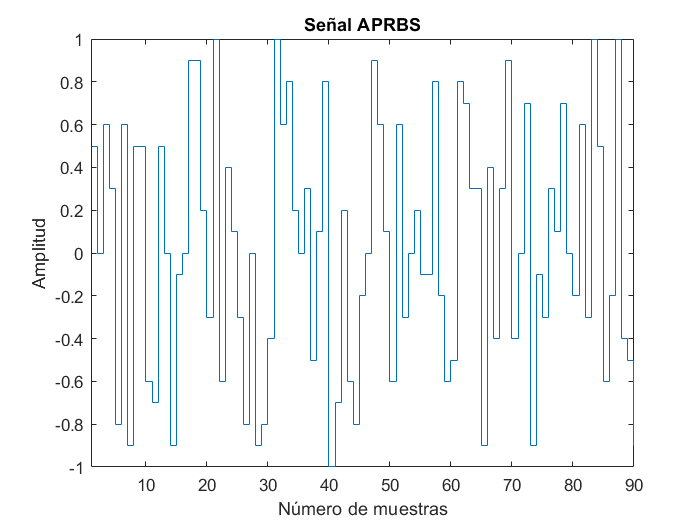
\includegraphics[width=10cm,height=7cm]{imag/APRBS}
\caption{Señal APRBS con Amplitud entre -1 y +1.}
\label{f_APRBS}
\end{figure}

\begin{figure}
\centering
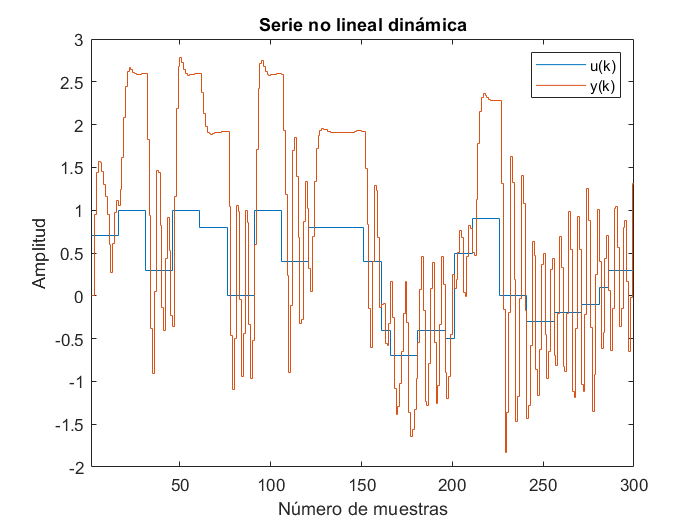
\includegraphics[width=10cm,height=7cm]{imag/SerieNoLineal}
\caption{Respuesta de la serie no lineal.}
\label{f_SerieNoLineal}
\end{figure}

Una vez obtenidos los datos experimentales de entrada-salida, éstos son clasificados en tres conjuntos con distinta información: datos de entrenamiento, datos
de validación y datos de prueba; esto con el fin de evaluar adecuadamente los modelos
generados. El conjunto de entrenamiento se utiliza para determinar los parámetros del
modelo. El conjunto de prueba permite comparar distintas estructuras de los modelos
generados. Finalmente, el conjunto de validación permite verificar el sobreajuste del
modelo óptimo obtenido, evaluándolo en un nuevo conjunto de datos (distintos a los
datos del conjunto de entrenamiento y validación), analizando su capacidad de
generalización. En este caso se utiliza una división de 55\% de los datos para entrenamiento, 25\% para prueba y 20\% validación.

\subsection{Modelo lineal}

En este caso, supondremos que se ajustará un modelo lineal suponiendo que el sistema real es lineal con ruido blanco gaussiano aditivo, es decir,


\begin{equation}
y(k)=a_1 y(k-1)+a_2 y(k-2)+b_1 u(k-1)+b_2 u(k-2)+e(k)
\label{e_ModeloLineal}
\end{equation}

Luego, se propone un modelo lineal para llevar a cabo la predicción a 1 paso, de modo tal que:

Predicción a 1 paso:

\begin{equation}
\hat{y}(k)=\hat{a}_1 y(k-1)+\hat{a}_2 y(k-2)+\hat{b}_1 u(k-1)+\hat{b}_2 u(k-2)
\label{e_Pre1paso}
\end{equation}

Este modelo no considera un valor constante o bias dao el supuesto que el sistema es lineal con ruido blanco aditivo. En caso que se sospechara que existe un bias o tendencia (trend) en el sistema, se puede agregar otro vector de unos a la matriz de regresores (o matriz de información).

Para llevar a cabo la estimación de los parámetros del modelo se utilizó la técnica de mínimos cuadrados, es decir:

\begin{equation}
\hat{\theta}=(Xent^T*Xent)^{-1}*Xent^T*\hat{y}(k)
\label{e_AjustMinCuadrados}
\end{equation}


En que $\hat{\theta}=[\hat{a}_1 \quad \hat{a}_2 \quad \hat{b}_1 \quad \hat{2}_2]^T$ es el vector de parámetros y $Xent$ es la matriz de regresores con los valores de las $n$ muestras ordenados por filas.

Los valores que se obtuvieron de los parámetros fueron los siguientes:


\begin{equation}
\hat{\theta}=\left(
                \begin{array}{c}
                  \hat{a}_1  \\
                  \hat{a}_2  \\
                  \hat{b}_1  \\
                  \hat{b}_2  \\
                \end{array}
              \right)
=\left(
   \begin{array}{c}
     0.8601 \\
     -0.6930 \\
     0.9724 \\
     0.3486 \\
   \end{array}
 \right)
\label{e_ValoresCoeficientes}
\end{equation}

A continuación, en la Tabla \ref{t_NoLinealp1}, se presentan las métricas de bondad del ajuste o errores en los diversos conjuntos de datos, a saber, conjunto de datos de entrenamiento, prueba o test y validación.


% Table generated by Excel2LaTeX from sheet 'Sheet1'
\begin{table}[htbp]
  \centering
  \caption{Errores o Métricas de bondad de ajuste a 1 paso}
    \begin{tabular}{|p{4.055em}|r|r|r|}
    \toprule
    Métricas & \multicolumn{1}{p{6.11em}|}{Conjunto Entrenamiento} & \multicolumn{1}{p{5.61em}|}{Conjunto de Prueba} & \multicolumn{1}{p{5.055em}|}{Conjunto de Validación} \\
    \midrule
    RMSE  & 0.0115 & 0.019 & 0.0241 \\
    \midrule
    MAPE  & 123.1323 & 101.9383 & 169.4761 \\
    \midrule
    MAE   & 0.3313 & 0.3402 & 0.3524 \\
    \bottomrule
    \end{tabular}%
  \label{t_NoLinealp1}%
\end{table}%

\subsection{Modelo difuso Takagi-Sugeno Tipo-1}

Para seleccionar las variables que actúan como entrada al sistema difuso, se realiza un análisis de sensibilidad. Suponiendo una estructura del modelo inicial difuso con 8 variables de entrada $y(k-1)$,... $y(k-4)$, $u(k-1)$,...,$u(k-4)$. En la Fig. \ref{f_P1Sensibilidad} se muestran los índices de las sensibilidades del modelo inicial para las 8
variables de entrada, comprobándose que las variables las variables $y(k-3)$, $y(k-4)$, $u(k-1)$ y $u(k-4)$ presentan menores índices de las sensibilidades, por lo cual no son incluidos en el modelo difuso.

\begin{figure}
\centering
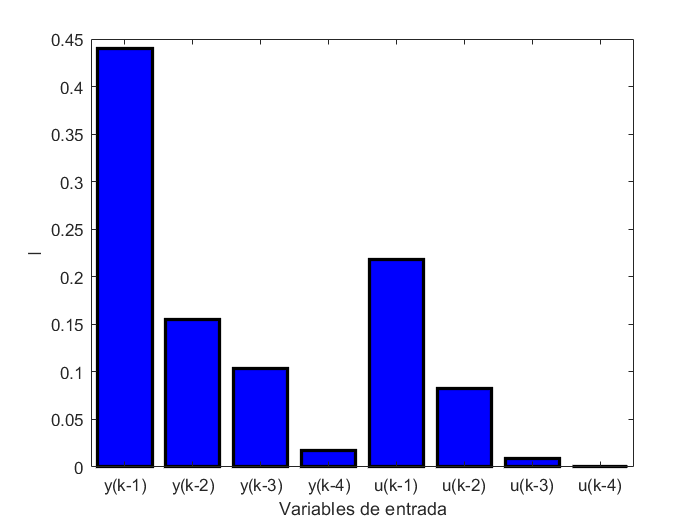
\includegraphics[width=10cm,height=7cm]{imag/P1Sensibilidad}
\caption{Índice de Sensibilidades.}
\label{f_P1Sensibilidad}
\end{figure}

La Tabla \ref{t_Error} indica el valor del Error Cuadrático Medio (MSE) para los modelos encontrados.


\begin{equation}
MSE=\frac{1}{N}\sum_{k=1}^{N}(y(k)-y_{fuzzy}(k))^2
\label{e_MSE}
\end{equation}

donde $N$ es la cantidad total de datos, $y(k)$ es la salida de la planta real en el instante , e $y_{fuzzy}(k)$ es la predicción realizada por el modelo difuso en el instante .

% Table generated by Excel2LaTeX from sheet 'Sheet1'
\begin{table}[htbp]
  \centering
  \caption{Valores de los Índices de Error Utilizando Análisis de Sensibilidades.}
    \begin{tabular}{|r|l|r|}
    \toprule
    \multicolumn{1}{|p{4.055em}|}{Modelo } & \multicolumn{1}{p{5.555em}|}{Variables de entrada } & \multicolumn{1}{p{4.055em}|}{MSE} \\
    \midrule
    1     & $y(k-1)$,$y(k-2)$,$y(k-3)$,$y(k-4)$, $u(k-1)$,$u(k-2)$,$u(k-3)$,$u(k-4)$     & 0.1517 \\
    \midrule
    2     & $y(k-1)$,$y(k-2)$,$u(k-1)$,$u(k-2)$    & 0.0902 \\
    \bottomrule
    \end{tabular}%
  \label{t_Error}%
\end{table}%

La optimización de la estructura del modelo difuso consiste principalmente en determinar el número óptimo de reglas del modelo difuso. En este caso se definió un número máximo de 11 clusters y se entrenó el modelo para cada una de las posibles valores de clusters.

La Fig. \ref{f_P1reglas11} muestra la Raíz del Error Cuadrático Medio (RMSE) para los conjuntos de entrenamiento y prueba.  Si no importa la complejidad, el mejor modelo es aquel que
tiene menor RMSE. Sin embargo, es posible que un modelo con peor índice de
desempeño, pero menos complejo que el modelo óptimo, pueda obtener resultados
aceptables bajo un estándar de rendimiento definido preliminarmente. Por lo antes expuesto para este problema se escoge como número de clusters 5, por lo que el modelo difuso contará con 5 reglas.

\begin{equation}
MSE=\sqrt{\frac{1}{N}\sum_{k=1}^{N}(y(k)-y_{fuzzy}(k))^2}
\label{e_RMSE}
\end{equation}



\begin{figure}
\centering
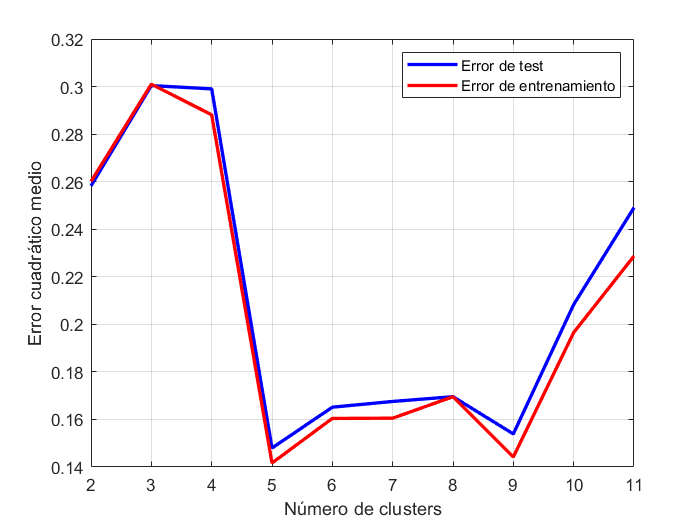
\includegraphics[width=10cm,height=7cm]{imag/P1reglas11}
\caption{Índice de Sensibilidades.}
\label{f_P1reglas11}
\end{figure}

\begin{figure}
\centering
\caption{Clusters.}
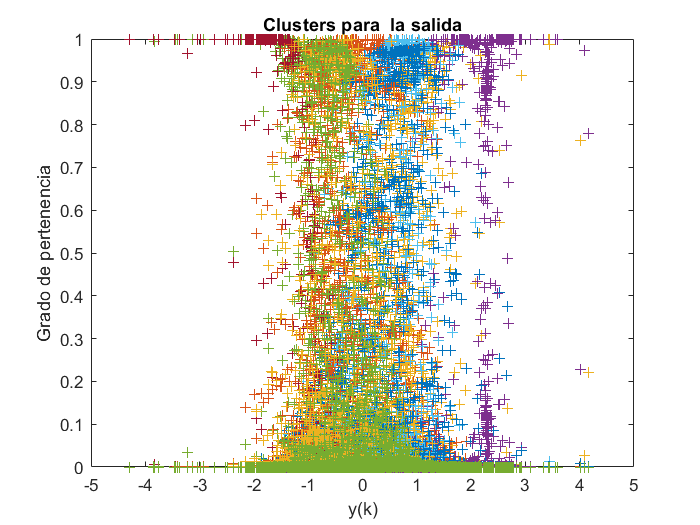
\includegraphics[width=7cm]{imag/ClusterSalida}\\
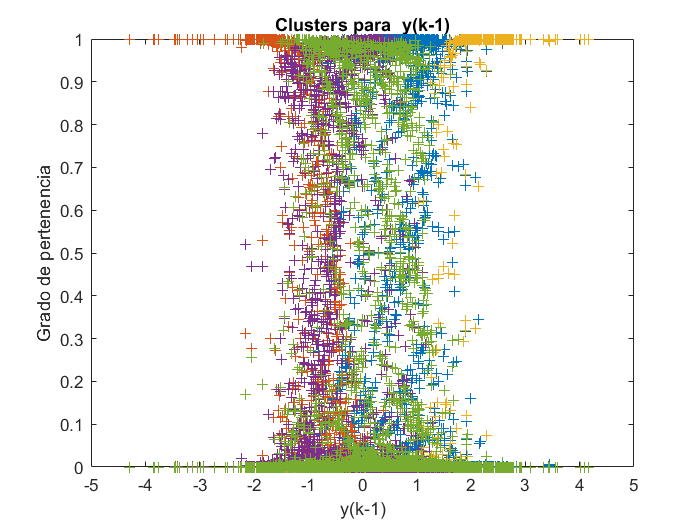
\includegraphics[width=7cm]{imag/Clustery1}
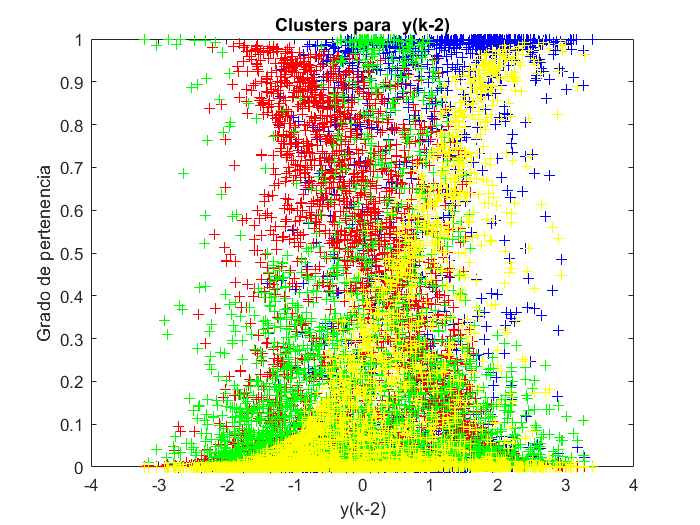
\includegraphics[width=7cm]{imag/Clustery2}\\
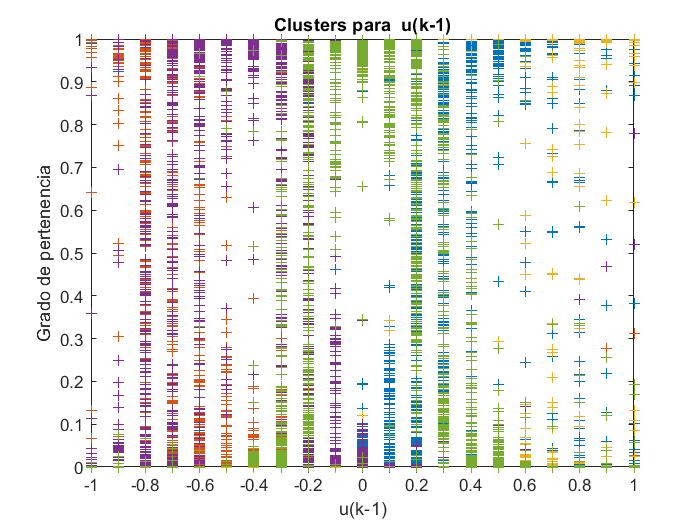
\includegraphics[width=7cm]{imag/Clusteru1}
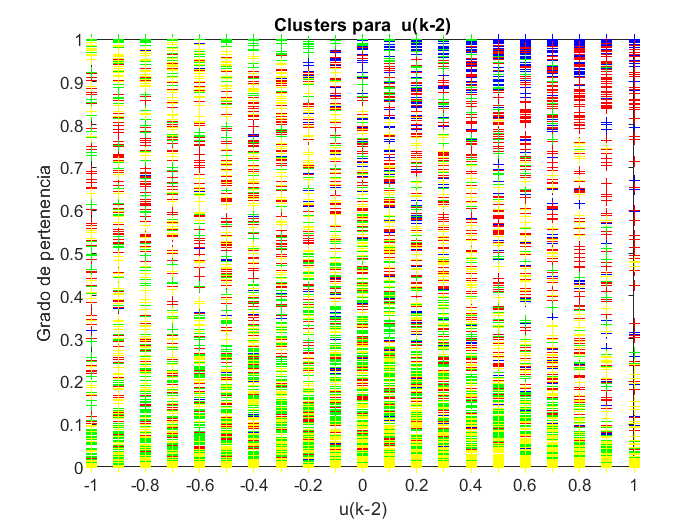
\includegraphics[width=7cm]{imag/Clusteru2}\\
\label{f_Cluster}
\end{figure}

\begin{figure}
\centering
\caption{Salida del modelo.}
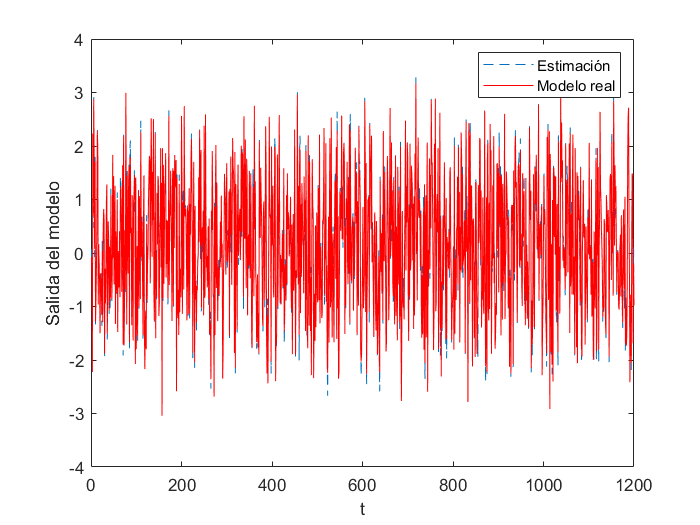
\includegraphics[width=7cm]{imag/P1Salida}
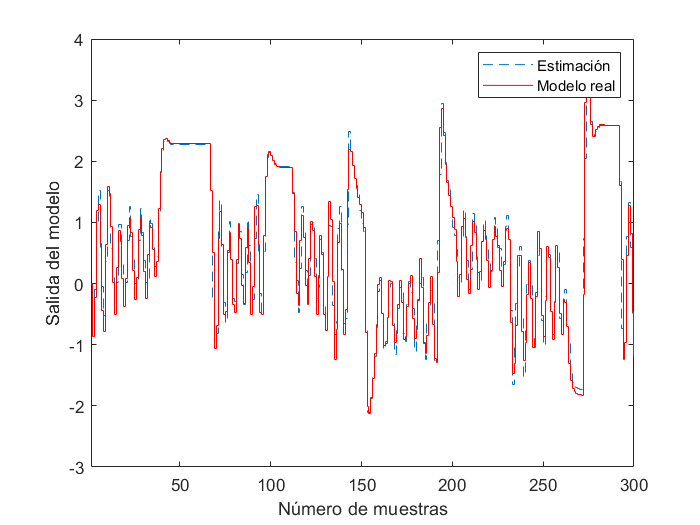
\includegraphics[width=7cm]{imag/P1SalidaZoom}
\label{f_SalidaModelo}
\end{figure}

\begin{figure}
\centering
\caption{Salida del modelo a 1 paso.}
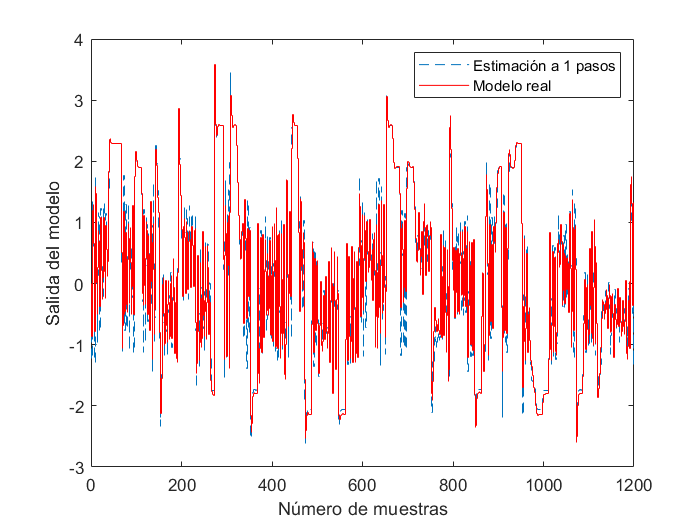
\includegraphics[width=7cm]{imag/P1Salida_p1}
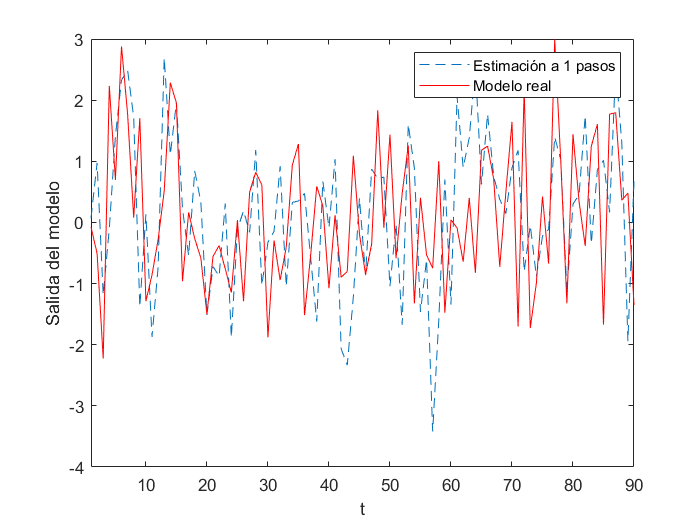
\includegraphics[width=7cm]{imag/P1Salida_p1Zoom}
\label{f_SalidaModelop1}
\end{figure}

\begin{figure}
\centering
\caption{Salida del modelo a 8 paso.}
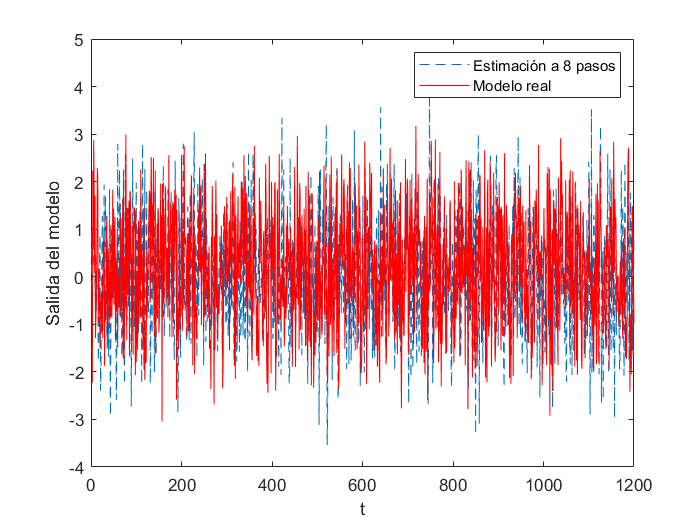
\includegraphics[width=7cm]{imag/P1Salida_p8}
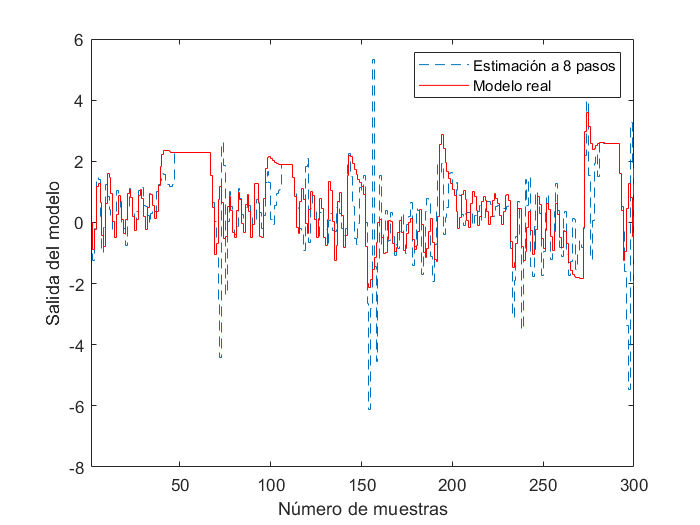
\includegraphics[width=7cm]{imag/P1Salida_p8Zoom}
\label{f_SalidaModelop8}
\end{figure}

\begin{figure}
\centering
\caption{Salida del modelo a 16 paso.}
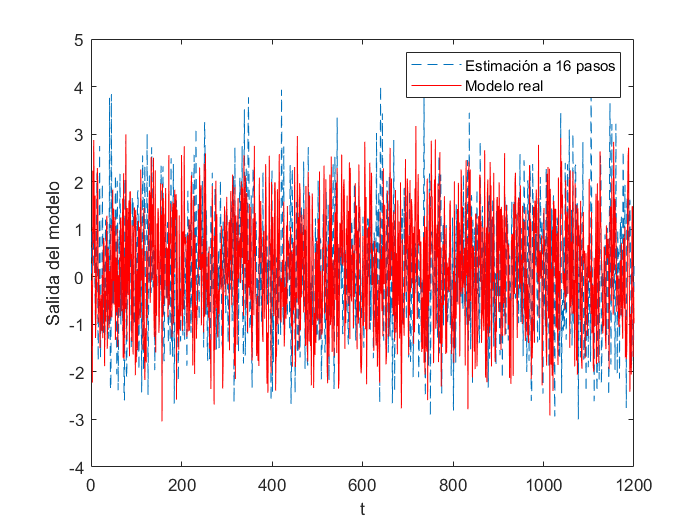
\includegraphics[width=7cm]{imag/P1Salida_p16}
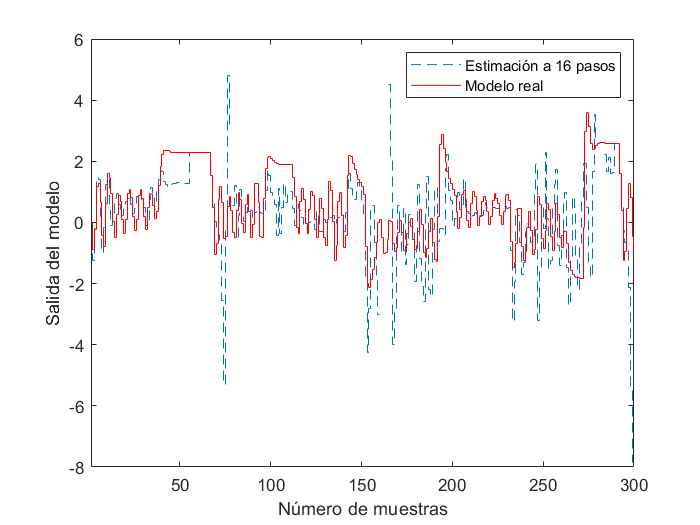
\includegraphics[width=7cm]{imag/P1Salida_p16Zoom}
\label{f_SalidaModelop16}
\end{figure}

% Table generated by Excel2LaTeX from sheet 'Sheet1'
\begin{table}[htbp]
  \centering
  \caption{Métricas para el Modelo Difuso}
    \begin{tabular}{|l|r|r|r|r|}
    \toprule
    Modelos & \multicolumn{1}{l|}{Estimado} & \multicolumn{1}{p{6em}|}{Predicción a 1 pasos} & \multicolumn{1}{p{6.39em}|}{Predicción a 8 pasos} & \multicolumn{1}{p{5.445em}|}{Predicción a 16 pasos} \\
    \midrule
    RMSE  & 0.0044 & 0.01104 & 0.0959 & 0.0105 \\
    \midrule
    MAPE  & 37.61 & 402.84 & 428.11 & 393.38 \\
    \midrule
    MAE   & 0.1038 & 1.1249 & 1.2392 & 1.2769 \\
    \bottomrule
    \end{tabular}%
  \label{tab:addlabel}%
\end{table}%




%\section{Problema 2}
%Para la operación óptima de las micro-redes es importante contar con modelos de predicción confiables de variables tales como: potencia solar, potencia eólica, consumo, estado de carga de las baterías, entre otras variables. Los modelos e intervalos de predicción son importantes debido a la incertidumbre asociada a la generación con energía renovable y la variabilidad del consumo local.
%
%Por tal razón, se le ha confiado a usted el proyecto de determinar modelos de predicción para la generación de energía en un sistema fotovoltaico instalado en una cierta comunidad del norte del país. La finalidad de este proyecto es la de disponer de información futura de generación fotovoltaica, para así poder gestionar el funcionamiento del resto de los elementos que componen a la micro-red.
%
%Para esto se le entregarán datos históricos de generación fotovoltaica (expresada en KW) medida en la comunidad durante el periodo septiembre-diciembre de los años 2015 y 2017. Estos datos tienen un tiempo de muestreo de 1 hora (considerar porcentajes adecuados de los datos en las fases de training, test y validación).
%
%Como usted sabe, son varias las formas que se pueden emplear para la modelación a partir de estos datos, por lo que debe seleccionar el tipo de modelo más adecuado para dicha aplicación.
%
%Se sugiere considerar los datos del año 2015 como base de entrenamiento y las mediciones del año 2017 como base de prueba y validación. Para este trabajo se le pide detallar la metodología utilizada para:
%
%\begin{enumerate}[a)]
%  \item Obtener dos modelos de predicción (a elección entre los vistos en este curso) y evaluar las predicciones a 1, 6 y 12 pasos. Comparar el desempeño de todos los modelos a partir de las métricas más apropiadas tales como RMSE, MAPE, MAE, entre otras.
%  \item Construir un intervalo de predicción para los modelos obtenidos en a), utilizando método que ud. seleccione.
%\end{enumerate}
%
%\subsection{Selección de Datos}
%Se cuenta con los datos históricos de generación fotovoltaica (expresada en KW) medida en la comunidad durante el periodo septiembre-diciembre de los años 2015 y 2017. Para la selección de los conjuntos de entrenamiento, prueba y validación se utiliza una división $[60\%,20\%,20\%]$, tomándose en este caso 2160 muestars del año 2015 para entrenamiento, que corresponde a 90 días de simulaciones, y para prueba y validación 720 muestras del año 2017, el equivalente a 30 días.





\newpage
\section{Conclusión}


\newpage
\bibliographystyle{IEEEtran}
\bibliography{biblio}
\end{document} 